% Paper B — the replication paper. Skeleton, 2026-09-21.
%
% Conventions for this draft:
%   \todo{...}   something still to be written, decided or checked
%   \src{...}    where a number comes from (doc, command); remove before submission
% Every number in this file is copied from the repository documents named in
% CLAIMS.md at tag replication-v1; none is typed from memory. If a document
% changes, change CLAIMS.md first, then this file.
\documentclass[11pt,a4paper]{article}
\usepackage[T1]{fontenc}
\usepackage[utf8]{inputenc}
\usepackage{lmodern}
\usepackage[margin=2.6cm]{geometry}
\usepackage{microtype}
\usepackage{graphicx}
\usepackage{booktabs}
\usepackage{tabularx}
\usepackage{xcolor}
\usepackage{caption}
\usepackage[round]{natbib}
\usepackage[hidelinks,colorlinks=false]{hyperref}
\usepackage{url}

\graphicspath{{../../docs/replication/figures/}{figures/}}

\newif\ifdraft \drafttrue
\ifdraft
  \newcommand{\todo}[1]{\textcolor{red!70!black}{[\textsc{todo:} #1]}}
  \newcommand{\src}[1]{\textcolor{blue!50!black}{\footnotesize\,[#1]}}
\else
  \newcommand{\todo}[1]{}
  \newcommand{\src}[1]{}
\fi
\newcommand{\arm}[1]{\texttt{#1}}
\newcommand{\sig}[1]{\textbf{#1}} % interval excludes zero

\title{A 2004 Model of Visual Attention, Reimplemented and Re-tested by Its Author%
\thanks{Code, configurations, and every command behind the numbers reported here:
\url{https://github.com/gerriet/visual-attention}, tag \texttt{replication-v1}.}}
\author{Gerriet Backer\\ \small\todo{affiliation / independent researcher; e-mail}}
\date{\todo{date}}

\begin{document}
\maketitle

\begin{abstract}
In 2004 I submitted a dissertation that proposed a two-stage model of visual
attention for active vision: a bottom-up stage of region-based features and a
neural field, and a symbolic second stage that tracks a few \emph{object files}
and inhibits return to \emph{objects} rather than to locations. Its central
claim---that object-based inhibition of return is what a serial attention system
needs in a dynamic scene---rested on one simulation experiment without
intervals and on demonstrations. Twenty years later I reimplemented the model and tested it again: 24 of the thesis's own
experimental findings (among them its one quantitative test of the central claim), that claim under a protocol with predictions
committed before each confirmatory run, and its scanpaths against human gaze.
\todo{update the count when replication-v2 is tagged: 25 findings, 22 replicated, 3 in part.}
Twenty-two findings replicate and two replicate in part. The central claim holds:
on 30 fresh scenes per regime, object-based inhibition reaches new objects sooner
and keeps cycling through a scene more evenly than space-based inhibition, also
against a motion-compensated spatial baseline and under two parameter sets.
\todo{one sentence on the real-video check once it has run.}
On still images the model's scanpaths are only slightly better than chance and
do not beat a constant central path, which the thesis never claimed they would.
The more general result is about replication itself. A first, approximate
reimplementation \emph{refuted} the central claim, robustly and for reasons that
looked principled; the refutation was an artefact of two infidelities---a
symmetry feature that normalised where the original thresholded, and neural
field parameters taken from a function's defaults rather than from the deployed
system. Both were found only by re-running the thesis's own small experiments,
not by the downstream benchmark that they corrupted.
\end{abstract}

% ---------------------------------------------------------------------------
\section{Introduction}
\label{sec:intro}

\todo{Opening paragraph: what the dissertation was, in two sentences a reader
outside attention modelling can follow \citep{backer2004}. Cite the two earlier
English-language publications of the model \citep{backer2001,backer2003}, since the
thesis is in German.}

\todo{Why re-test now. (i) The claim's only quantitative support is the
world-model experiment of thesis \S9.2 \citep[Fig.~5]{backer2003}: simulated
master maps, 50 runs per condition, means without intervals, one hand-set
baseline. (ii) The idea---a small symbolic world model that
decides where an expensive serial process looks next---has a new use as a
front-end for models with a token budget; that use needs the claim to be true.
Keep (ii) to two sentences: it is the subject of separate work and not evaluated
here.}

\paragraph{What this paper is, and is not.} It is a reimplementation and a
re-test by the original author, with access to the thesis text and to part of the
original source code. It is not an independent replication, and the difference
matters in both directions: I could resolve ambiguities that an outsider could
not, and I had every incentive to find that my own thesis was right. The
protocol in Section~\ref{sec:protocol} is built around the second point. The
original sources cannot be released (I do not hold the rights); what was taken
from them is reported as facts---parameter values, algorithmic steps---in
Section~\ref{sec:sources} and Appendix~\ref{app:params}.

\paragraph{Contributions.}
\begin{enumerate}
  \item A replication dossier: 24 experimental findings of the thesis, each
        rebuilt, measured and given a verdict (22 replicated, 2 partially), all
        regenerated by one command (Section~\ref{sec:dossier}).
  \item A confirmatory test of the thesis's central claim, object-based versus
        space-based inhibition of return in dynamic scenes, with a strengthened
        baseline, fresh scenes and predictions committed before the run
        (Section~\ref{sec:h1}). \todo{+ real video.}
  \item An evaluation of the model's scanpaths against human gaze on MIT1003,
        with two methodological findings about scoring scanpaths
        (Section~\ref{sec:h4}).
  \item A case study in how a reimplementation goes wrong: a negative result
        that survived three rounds of honest analysis and was about the
        reimplementation, not the model (Section~\ref{sec:discussion}).
\end{enumerate}

% ---------------------------------------------------------------------------
\section{The 2004 model}
\label{sec:model}

\todo{One figure: the two stages (redraw thesis Abb.\ \todo{number}; own figure,
no rights issue). Half a page of text per stage. Keep equations to those the
dossier tests against: eq.~5.6 (eccentricity), 5.12 (sigmoid), 5.13--5.16
(stereo), the exclusivity weighting, the field equation.}

\subsection{Stage one: region-based features and a neural field}
\begin{itemize}
  \item \textbf{Colour contrast.} Transform to a perceptually uniform space
        (the mathematical transform to Munsell, \citealp{miyahara1988}); region
        growing with a variance-dependent threshold; contrast of each region to
        its neighbours weighted by shared border; a sigmoid.
  \item \textbf{Eccentricity.} Edge-bounded regions; second-order central
        moments; $\varepsilon = \frac{(m_{20}-m_{02})^2 + 4m_{11}^2}{(m_{20}+m_{02})^2}$
        \citep{jaehne}, 0 for a round region, 1 for a line.
  \item \textbf{Symmetry.} Boundary-based, after \citet{bollmann1997}: Gabor edge
        energy in 12 orientations summed in pairs of boxes on opposite sides of a
        point, over radii 6--15 at three scales (thesis Tab.~5.1).
  \item \textbf{Depth} from a rectified stereo pair: windowed normalised
        cross-correlation of Gabor magnitudes at a few near-vertical
        orientations over a disparity range, spatially integrated, winner-take-all
        per pixel (eq.~5.13--5.16); and \textbf{onset} for image sequences.
  \item \textbf{Exclusivity.} A feature value shared by $n$ regions is divided
        by $c^{\,n}$, $c = 1.1$: common is less salient than unique.
  \item \textbf{Selection} by a two-dimensional neural field of the Amari type
        \citep{amari1977}: local excitation, broad and global inhibition; the
        clusters of activation that survive are the candidates handed to stage
        two. The field, not a fixed count, decides how many there are.
\end{itemize}
\todo{Relate to the saliency-map lineage \citep{treisman1980,koch1985,itti1998}
in one paragraph: what is shared (parallel feature maps, fusion, a selection
dynamics), what differs (regions rather than centre--surround pixels; absolute
rather than min--max-normalised feature scales; a field that returns several
clusters).}

\subsection{Stage two: object files and inhibition of return on objects}
\todo{Object files \citep{kahneman1992}; a handful of tracked entities
\citep{pylyshyn1988}; correspondence by nearest centroid; behaviours that choose
the focus among object files; inhibition of return \citep{posner1984,klein2000}
attached to the object file, so that it moves with the object
\citep{tipper1991}. The claim to be tested: in a dynamic scene this beats
inhibiting locations. Related computational work on object-based attention:
\citet{sun2003,walther2006} \todo{literature pass 2005--2026: proto-object models,
object-based IOR in computational models, multi-object tracking as attention}.}

% ---------------------------------------------------------------------------
\section{Reimplementation and protocol}
\label{sec:method}

\subsection{The reimplementation}
C++17 and OpenCV, with a Python evaluation layer; every component is selected by
a configuration file, and every model emits one interchange format, which is all
the evaluation code reads. The replication is defined as a set of configuration
profiles (\texttt{configs/thesis/}) that may enable dissertation components only
(enforced by a test), plus fidelity tests and behavioural goldens. It is frozen
at the tag \texttt{replication-v1}; later work on a modernised system adds
sibling components and does not edit these. \src{docs/adr/0005}
\todo{Disclose how the code was written: the reimplementation was developed by
the author with an AI coding assistant (Claude Code). Word this as the venue's
policy requires; say what was checked by hand---the ports against the sources,
every verdict in the dossier, every prediction.}

\subsection{Sources of truth, and what cannot be shown}
\label{sec:sources}
Three sources, in order of authority for this paper:
\begin{enumerate}
  \item \textbf{The thesis text} (open access, in German) is what a reader can
        check, so the documented replication profile follows the text wherever
        text and code disagree.
  \item \textbf{The surviving original sources} (2003--2005, C++) cover the
        static features, the stereo feature, the neural fields and the program
        that configured the dissertation system. They settled what the text
        leaves open---most importantly the field's parameters, which the thesis
        describes only qualitatively. They cannot be published. Appendix~\ref{app:params}
        lists every value taken from them, next to the text's.
  \item \textbf{The thesis's figures}, as behavioural targets: the replication
        bar is loose behavioural equivalence, not pixel equality. The thesis's
        laboratory images did not survive, except the running example of
        Abb.~5.8--5.22; stimuli were rebuilt from the figures' descriptions.
\end{enumerate}
Where the two disagree, a second profile carrying the deployed system's values
is kept runnable, and Section~\ref{sec:textcode} compares them.

\subsection{Protocol}
\label{sec:protocol}
The rules below were adopted after an internal review found that earlier results
in this project had been tuned and tested on the same few seeds.
\src{docs/CRITICAL\_REVIEW\_2026-09.md, docs/HYPOTHESIS\_CLOSURE\_PLAN.md}
\begin{itemize}
  \item \textbf{Development and test data are disjoint.} Scenes with seeds 0--9
        shape the instrument; confirmatory runs use fresh blocks (1000--1029,
        2000--2029, 3000--3029), generated only after the predictions are
        committed.
  \item \textbf{Predictions are committed to the repository before the run},
        with a refutation criterion each (H1: commit \texttt{ab7d75e}; human
        gaze: \texttt{36761d8}). This is a public, timestamped record, not a
        registration with a third party.
  \item \textbf{The arm expected to lose gets a strengthened version}, and every
        comparison a trivial baseline.
  \item \textbf{Paired bootstrap} over independent units (scenes, images), 4000
        resamples, 95\% intervals; a difference ``holds'' if its interval
        excludes zero.
  \item \textbf{Verdicts} for the dossier: \emph{replicated} (holds, measured),
        \emph{partially}, \emph{diverged} (with the reason), \emph{not attempted}
        (with the reason).
\end{itemize}

% ---------------------------------------------------------------------------
\section{Study 1: the thesis's own experiments}
\label{sec:dossier}

The thesis supports its features and its selection stage with small experiments:
vary the property a feature is named after and watch the response; add noise;
sweep a parameter and find the range in which the result stays plausible. Each
was rebuilt. Feature responses are read on an absolute $[0,1]$ scale, one feature
at a time. Table~\ref{tab:dossier} gives the verdicts; all numbers are printed by
\texttt{eval/replication.py --all} (CPU, about 15 minutes).
\src{docs/replication/REPLICATION\_DOSSIER.md}

\begin{table}[t]
\caption{The 24 findings. ``Sys.\ param.''\ = replicated with the deployed
system's field parameters and diverged with the ones the port first used
(Finding~B). ``After port'' = diverged before the symmetry feature was ported
from the original, replicated after (Finding~A).}
\label{tab:dossier}
\footnotesize
\begin{tabularx}{\linewidth}{@{}llXl@{}}
\toprule
\# & Thesis & Claim & Verdict \\
\midrule
1  & Abb.~5.10 & Eccentricity is 0 for round and high for elongated shapes & replicated \\
2a & Abb.~5.13 & Stretching an object raises eccentricity monotonically & replicated (eq.~5.6 $\pm$0.02) \\
2b & Abb.~5.13 & \ldots and lowers symmetry & replicated, after port \\
3a & Abb.~5.14 & Eccentricity maximum stays on its object under noise & replicated to $\sigma\approx38$ \\
3b & Abb.~5.14 & Symmetry maximum stays on its object under noise & replicated, after port \\
4  & Abb.~5.15 & Segmentation plausible for growth threshold 0.5--0.75 & \emph{partially} \\
5  & Abb.~5.16 & \ldots and for merge threshold 12--36 & replicated ($r\ge0.88$ over 4--48) \\
6  & Abb.~5.20 & Colour contrast grows with colour difference & replicated \\
7  & Abb.~5.21 & Colour-contrast maximum robust to noise & replicated \\
8  & Abb.~5.22 & Insensitive to \texttt{cc\_add}/\texttt{cc\_mult} over a broad range & replicated \\
9  & Abb.~5.34 & Exclusivity lowers common against unique values & replicated \\
11 & Abb.~5.28 & Depth response follows distance & replicated (exact) \\
12 & Abb.~5.29 & Depth is found in a random-dot stereogram & replicated \\
13 & Abb.~5.30 & Disparity estimate nearly unchanged under noise & replicated \\
14 & Abb.~5.31 & Several orientations help; beyond one the choice matters little & replicated \\
15 & Abb.~5.32 & Variance threshold: only extreme values hurt & replicated (synthetic) \\
15b& on Abb.~5.25 & Disparity correct ``in the great majority of regions'' & replicated on real pairs \\
16 & Abb.~6.4  & Field hysteresis between two inputs & replicated, sys.\ param. \\
17 & Abb.~6.5  & Bifurcation: two clusters from a certain distance & replicated \\
18 & Abb.~6.6  & Noise suppressed up to amplitude 1.2 for a pulse of 1 & replicated, sys.\ param. \\
19 & Abb.~6.8  & Stable state in about 10 cycles & replicated (10) \\
20 & Abb.~6.9  & Tracking in noise: $\sim$10 cycles per frame suffice within limits & replicated, sys.\ param. \\
21 & Abb.~6.10 & Approaching maxima: repulsion, merging below distance 5 & replicated, sys.\ param. \\
10 & Abb.~6.14 & Identity survives temporary occlusion & \emph{partially} \\
\bottomrule
\end{tabularx}
\end{table}

\subsection{Features}
\todo{Half a page. The quantitative anchors: eccentricity of a 2:1 ellipse 0.354
against eq.~5.6's 0.360, of an 8:1 bar 0.934 against 0.940; symmetry falling
0.67~$\to$~0.15 as the same object is stretched; colour contrast
0.00~$\to$~0.32~$\to$~0.81~$\to$~0.98~$\to$~1.00; exclusivity ratio 1.51 for five
bars against the predicted $1.1^4 = 1.46$. Figure~\ref{fig:ecc}. The side finding
on histogram equalisation and three-level synthetic images belongs here as a
warning about synthetic stimuli.}

\begin{figure}[t]
\centering
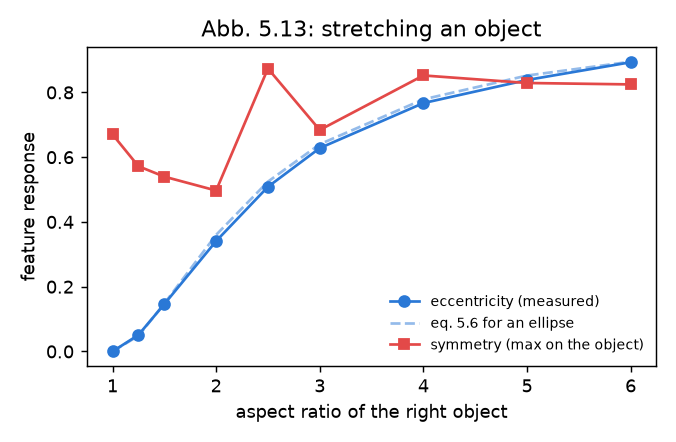
\includegraphics[width=.62\linewidth]{ecc_variation.png}
\caption{Thesis Abb.~5.13 rebuilt: an object of constant area is stretched from
1:1 to 6:1. Eccentricity rises on the curve of eq.~5.6; symmetry falls. Before
the symmetry feature was ported from the original it \emph{rose}
(0.67~$\to$~0.82). \todo{redraw for print: vector, one column, fonts.}}
\label{fig:ecc}
\end{figure}

\paragraph{The two partial verdicts.} The growth threshold (Abb.~5.15) is stable
in the range the thesis names, but the map correlation with the default is only
0.64--0.78 there; ``plausible'' in the thesis is a visual judgement and a
pixel-wise correlation is a stricter reading. Identity through occlusion
(Abb.~6.14) is tracked in the object files here, not in the fields, so the figure
is not reproduced as such; the question is measured in Section~\ref{sec:h1}
(occlusion regime, Table~\ref{tab:h1}: 2.8 labels per attended object with
position-only correspondence, 1.5 with feature-led revival of inactive object
files, which is what thesis \S7.2.3 describes). \todo{revisit this verdict: with
the correspondence the thesis specifies it may be ``replicated''.}

\subsection{Depth}
\todo{Synthetic pairs with known disparity: exact recovery for $d=0\ldots14$;
9.91 of 10~px at noise $\sigma\approx90$ grey levels---\emph{without} the
multi-scale scheme the thesis credits for the robustness, which is not ported: the
finding replicates, the thesis's explanation is untested. Then the independent
check on three Middlebury pairs \citep{scharstein2002}: 82--85\% of pixels within
1~px at the default threshold; raising the threshold never reduces wrong pixels,
it only discards correct ones. Note the corrected first reading (a synthetic band
of pure noise suggested raising the threshold; real pairs say the opposite).
Figure: \texttt{stereo\_real\_threshold.png}.}

\subsection{Finding A: a symmetry feature that answered beside its objects}
\label{sec:findingA}
For a single bright disk on a grey ground, the first reimplementation's symmetry
map responded inside the disk \emph{and equally strongly about 80~px to either
side of it}; the global maximum lay off the object for every disk size tried,
without noise. The summation core was a faithful port. What differed was what
followed it: the original works on an absolute scale---edge magnitudes clipped,
then a fixed offset (60 of 255) subtracted from every radius band---which removes
the response that an edge on \emph{one} side alone produces---the sum over the
two boxes is additive, so such a response is a substantial fraction of a closed
contour's \todo{measure the ratio on the ported feature and state it}. The reimplementation had instead normalised each band to its
own maximum and applied relative thresholds. With no absolute reference, a
one-sided response is as strong as a true centre and appears as a ring around
every object. After porting the combination step, a lone disk peaks at its centre
(0.43 / 0.82 / 0.99 for radius 12 / 24 / 40) and a single straight edge gives
0.08. One thing the sources do not settle is the gain of the original Gabor
implementation, which fixes what ``60 of 255'' means; the calibration chosen (a
full-contrast step edge has energy 1) is a reconstruction.
\src{dossier, finding A; symmetry\_feature.h}

\subsection{Finding B: field parameters from a function's defaults}
\label{sec:findingB}
The port had taken the neural field's parameters from the \emph{default
arguments} of the original's setter functions. The program that configured the
dissertation system set different ones: a narrower excitatory centre, a separate
broad inhibitory surround, and eight times the global inhibition, on a
$64\times64$ field (Appendix~\ref{app:params}). Table~\ref{tab:field} shows the
thesis's field experiments \citep[published in English as][]{backer2002} under both.

\begin{table}[t]
\caption{Field dynamics (thesis Abb.~6.4--6.10) under the deployed system's
parameters and under the defaults the port first used. Inputs are Gaussian blobs
($\sigma=3$~px); the thesis does not give the shape of its input peaks, and the
distances depend on that choice to some degree.}
\label{tab:field}
\footnotesize
\begin{tabularx}{\linewidth}{@{}XXXX@{}}
\toprule
Experiment & Thesis & System's parameters & Port's defaults \\
\midrule
Two approaching maxima (6.10) & repulsion, merging below distance 5, no oscillation
  & two clusters down to 6, one from 5; pushed apart 3--5~px; one clean transition
  & never merge ($\ge20$~px apart even when the inputs coincide) \\
Separating again (6.5/6.10) & re-split only beyond that distance & re-split at 13 & split at 19 \\
Noise around a pulse of 1 (6.6) & only signal-caused activation up to 1.2
  & 0.000 outside the pulse up to 1.2; 0.7\% at 1.4 & 1.4\% at 0.8 \\
Hysteresis $\alpha$ / $1-\alpha$ (6.4) & switch only when clearly stronger
  & switches at 0.55 rising, holds to 0.25 falling & switches at 0.35, before the inputs are equal \\
Convergence (6.8) & $\sim$10 cycles & 10 & 8 \\
Tracking in noise (6.9) & $\sim$10 cycles per frame within limits
  & yes for amplitude $\ge0.7$; limit at 0.5 and 10~px/frame
  & most targets at $\ge8$~px/frame lost \\
\bottomrule
\end{tabularx}
\end{table}

The noise experiment identifies the parameters about as sharply as a figure
without its data can: the thesis names an amplitude, 1.2, and with the system's
parameters the first activation outside the pulse appears at the very next step.
It also identifies the noise model (zero-mean). With the right parameters the
field decides how many fixations a scene deserves---four on average on MIT1003
images instead of always ten---which matters in Section~\ref{sec:h4}.
\todo{Figures: \texttt{field\_two\_maxima\_noise.png},
\texttt{field\_hysteresis\_tracking.png}; choose one for the main text.}

\subsection{Findings C--E: what a second source exposed}
\label{sec:findingsCDE}
The dossier was built from the thesis's chapters 5 and 6. Reading the last
English-language paper from the thesis work \citep{backer2003} against the thesis
and the code exposed three more gaps: (C) the thesis's own quantitative test of
its central claim had been overlooked (Section~\ref{sec:worldmodel}); (D) the
correspondence the reimplementation called ``the thesis's'' was position-only,
weaker than \S7.2.3; (E) object files were formed from saliency segments, not
from the field's activity clusters. All three were closed
(Sections~\ref{sec:worldmodel} and~\ref{sec:chain}). The surviving original
sources do not contain the second stage, so for it the thesis text and that paper
are the only record. \todo{Lesson for the discussion: a second description of the
same system, written for a different audience, is a cheap and effective fidelity
check.}

\subsection{Text or code?}
\label{sec:textcode}
\todo{A short paragraph and a compact version of the dossier's comparison table.
The text's and the deployed system's parameter sets differ in the eccentricity
and colour thresholds, exclusivity (1.1 vs.\ off) and the feature weights
(1/1/1 vs.\ 1.2/0.35/1.6). Neither is decisively better: the text's values are
the closer fit to the thesis's own equations (2:1 ellipse 0.35 vs.\ 0.19) and
slightly ahead on agreement with human scanpaths ($-0.016$ [$-0.023$, $-0.008$]
ScanMatch for code minus text); all other intervals include zero. H1 holds under
both (Section~\ref{sec:h1}). General point: when text and code disagree, report
both, and say which one the reader can check.}

% ---------------------------------------------------------------------------
\section{Study 2: object-based versus space-based inhibition of return}
\label{sec:h1}

\paragraph{The claim (H1).} In multi-object dynamic scenes, object-based
inhibition of return yields lower novel-object latency than space-based
inhibition and degrades gracefully with object speed. \todo{quote the thesis's
own formulation with page reference, in translation.}

\subsection{The thesis's own test}
\label{sec:worldmodel}
The thesis contains one quantitative test of its central claim (\S9.2; the main
result of \citealp{backer2003}), which the first version of the dossier, built
from chapters 5--6, had missed. Two models explore the same simulated master map
of attention and each keeps a world model---which object is where. Objects are
$5\times5$ pixels, static or moving on straight paths by at most 2~px per axis
and frame, at least 14~px apart, under uniform noise of half their amplitude;
1, 3 or 5 static and 0--5 dynamic objects; 50 runs of 40 frames per condition.
Recognition is simulated: it names the object under the focus after 3 frames
(conventional) or 4 (two-stage).
The \emph{conventional} model blurs, subtracts a decaying inhibition map ($8\times8$
marks, $\times0.8$ per frame) and takes the maximum; an identity stays bound to the
place where its object was selected. The \emph{two-stage} model is the thesis's
simplest variant---one 2D field of local inhibition, object files on its activity
clusters with the correspondence of \S7.2.3, the exploration behaviour---and an
identity moves with its object file. Measures: the mean number of objects whose
identity the world model holds within 20~px of the truth, and the mean position
error of those. What the sources leave open (map size, velocity distribution,
noise mean, when the conventional model's recognition looks at the focus) was
fixed on development seeds, the last in the conventional model's favour; two
variants were declared in advance; predictions were committed before the 50
confirmatory runs (\texttt{3edd62f}). \src{dossier, finding 22; eval/replication.py --only world-model}

\begin{figure}[t]
\centering
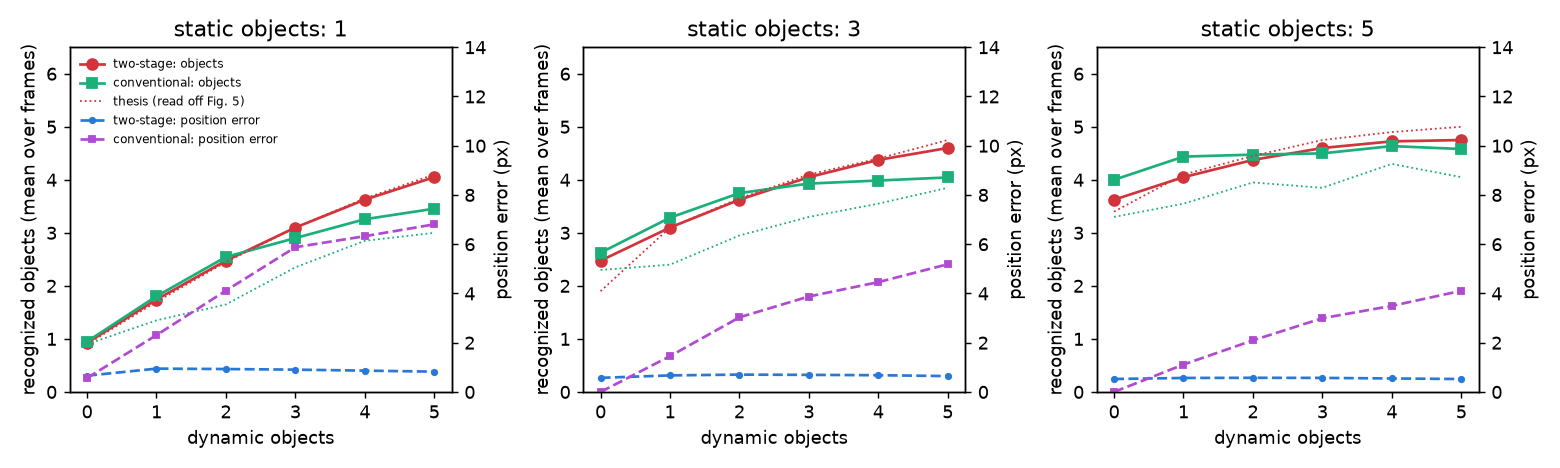
\includegraphics[width=\linewidth]{world_model.png}
\caption{Thesis Abb.~9.2 / \citet[Fig.~5]{backer2003} rebuilt: recognized objects
(left axes) and position error (right axes) for 1, 3 and 5 static objects. Dotted:
the thesis's curves, read off the published figure. \todo{redraw for print.}}
\label{fig:worldmodel}
\end{figure}

\paragraph{Result (Figure~\ref{fig:worldmodel}).} The two-stage model is within
0.01 of its optimum---every object recognized at the first opportunity and never
lost---in all 18 conditions, and its curve is the thesis's curve (within 0.25 in
17 of 18 conditions). The field produces exactly as many activity clusters as
there are objects in every condition. Its position error is 0.53--0.95~px; the
conventional model's grows with the number of moving objects to 4--7~px. Pooled
over the static counts, two-stage minus conventional recognized objects for 0--5
dynamic objects: $-0.18$, $-0.21$, $-0.10$, $+0.14$, $+0.28$, $+0.44$, every
interval excluding zero. So the thesis's scaling claim and its position-error
claim replicate in direction and size; two statements do not: ``ahead as soon as
anything moves'' (here: from three moving objects on) and ``below 0.5~px in every
condition''. The first is the baseline's doing: the conventional model rebuilt
from the description reaches its own optimum in static scenes (4.00 with five
objects) where the thesis's reached about 3.3, so the two-stage model's extra
frame per recognition is paid back later. Why the thesis's baseline fell short
the sources do not say. Four of five predictions held; the one about the variants
was half right (with recognition looking at the focus when it \emph{ends}, two
dynamic objects are a tie and the lead from three on grows to $+0.61$).

\paragraph{A third parameter finding.} Building this experiment exposed what
Finding~B had missed: over a stream the deployed system ran its field for a
\emph{fixed 20 cycles per frame} (its convergence test compared a summed change
with a threshold no noisy field meets) with an input gain of 0.765. With the
port's convergence test the field stops after about three cycles, a moving
object's cluster stays behind, self-sustained, and the object file stays with the
ghost.

This experiment measures what the system \emph{knows}; the study below measures
where attention \emph{goes}.

\subsection{Design}
Behaviours that are identical except in what they inhibit, over the same
features, fusion and object-file tracking (Table~\ref{tab:arms}); synthetic scenes
of coloured disks that move, bounce and are occluded, with ground truth; three
regimes: \emph{standard} (speed 6~px/frame, 60-px tag, one occlusion),
\emph{fast} (speed 40, 20-px tag), \emph{occlusion} (speed 20, 18-px tag,
10-frame occlusion); 40 frames; 30 scenes per regime.
\src{eval/dynamic\_ior.py --regime all --seeds 30 --seed0 2000; docs/DYNAMIC\_IOR\_STUDY.md}

\begin{table}[t]
\caption{Arms. \arm{spatial-ior-mc} is the strengthened version of the arm
expected to lose: its location tags drift with the velocity of the object they
were left on. The thesis's correspondence (\S7.2.3) uses position \emph{and}
feature similarity and revives inactive object files primarily by their
features; \arm{+aids} and \arm{+id} approximate that, the plain arm is weaker
than it. \todo{the project's documents call the plain arm ``the thesis's
correspondence'' and the others extensions; relabel there, and list the
differences of \arm{+id} from \S7.2.3: colour as the only feature, a summed
cost, no maximum age.}}
\label{tab:arms}
\small
\begin{tabularx}{\linewidth}{@{}lXX@{}}
\toprule
Arm & Inhibition rides on & Identity held by \\
\midrule
\arm{greedy} & nothing & --- \\
\arm{spatial-ior} & decaying location tags & --- \\
\arm{spatial-ior-mc} & location tags moving by dead reckoning & --- \\
\arm{object-ior} & object files & position only (an ablation of thesis \S7.2.3) \\
\arm{object-ior+aids} & object files & + motion prediction, feature similarity \\
\arm{object-ior+id} & object files & + feature-led revival of inactive files \\
\bottomrule
\end{tabularx}
\end{table}

\paragraph{Metrics.} Primary: \emph{latency}, the frames from an object's
appearance to its first fixation; and \emph{staleness}, the mean over all frames
and visible objects of the frames since that object was last attended. Staleness
was introduced for the confirmatory run because the revisit measure used during
exploration stops accruing once every object has been seen (after 2--8 of 40
frames) and is decided by a handful of fixations. Secondary: the share of
fixations on no object, and distinct labels per attended object (identity
switches). Coverage is 1.00 for every arm with inhibition and does not
discriminate.

\subsection{Three runs, and why the third one stands}
\label{sec:threeruns}
\todo{This subsection is the spine of the paper; write it carefully and without
hindsight polish.}
\begin{enumerate}
  \item \textbf{Exploration} (July--September; $\le6$ seeds, no intervals):
        space-based inhibition at least as good as object-based, ``usually
        better''. Explained at the time, plausibly, by tracking errors: object-based
        inhibition is only as good as its tracker. Recorded in the project as an
        honest negative result.
  \item \textbf{First confirmatory run} (seeds 1000--1029), after the colour and
        eccentricity features had been ported from the original: object-based
        inhibition wins on latency in all regimes, but not on staleness; a third
        of its fixations land on no object. Explained at the time, again
        plausibly, by segmentation: object files that are not objects.
  \item \textbf{Re-run} (seeds 2000--2029), after Study~1 had found and fixed the
        symmetry feature (Finding~A)---a change decided by a test that does not
        involve inhibition of return. Same command, same arms, same committed
        predictions.
\end{enumerate}

\begin{table}[t]
\caption{The re-run: 30 fresh scenes per regime. $\Delta$ is arm minus
\arm{spatial-ior}, paired over scenes, 95\% interval; \sig{bold} excludes zero.
Lower is better. Off-object share is 0.00 for every arm.}
\label{tab:h1}
\footnotesize
\begin{tabularx}{\linewidth}{@{}llrXrXr@{}}
\toprule
Regime & Arm & Lat. & $\Delta$ latency & Stal. & $\Delta$ staleness & Labels \\
\midrule
standard & \arm{greedy}          & 23.58 & \sig{+20.98} & 12.49 & \sig{+10.16} & 1.4 \\
         & \arm{spatial-ior}     &  2.61 &  &  2.33 &  & 1.7 \\
         & \arm{spatial-ior-mc}  &  2.46 & \sig{$-$0.15 [$-$0.32, $-$0.01]} & 2.06 & \sig{$-$0.27 [$-$0.41, $-$0.15]} & 1.7 \\
         & \arm{object-ior}      &  2.13 & \sig{$-$0.47 [$-$0.77, $-$0.24]} & 1.69 & \sig{$-$0.64 [$-$0.83, $-$0.47]} & 1.7 \\
         & \arm{object-ior+id}   &  2.10 & \sig{$-$0.51 [$-$0.82, $-$0.24]} & 1.67 & \sig{$-$0.66 [$-$0.86, $-$0.47]} & 1.3 \\
\addlinespace
fast     & \arm{greedy}          & 17.43 & \sig{+11.35} &  9.99 & \sig{+5.89} & 4.8 \\
         & \arm{spatial-ior}     &  6.08 &  &  4.10 &  & 4.3 \\
         & \arm{spatial-ior-mc}  &  3.37 & \sig{$-$2.72 [$-$4.13, $-$1.49]} & 2.78 & \sig{$-$1.32 [$-$1.84, $-$0.83]} & 4.6 \\
         & \arm{object-ior}      &  2.08 & \sig{$-$4.00 [$-$5.28, $-$2.86]} & 2.10 & \sig{$-$2.00 [$-$2.46, $-$1.59]} & 5.5 \\
         & \arm{object-ior+aids} &  1.73 & \sig{$-$4.36 [$-$5.63, $-$3.24]} & 1.75 & \sig{$-$2.35 [$-$2.81, $-$1.94]} & 3.9 \\
         & \arm{object-ior+id}   &  1.63 & \sig{$-$4.45 [$-$5.69, $-$3.36]} & 1.67 & \sig{$-$2.43 [$-$2.89, $-$2.02]} & 1.7 \\
\addlinespace
occlusion& \arm{greedy}          & 19.64 & \sig{+15.35} & 10.40 & \sig{+7.79} & 2.2 \\
         & \arm{spatial-ior}     &  4.29 &  &  2.61 &  & 2.4 \\
         & \arm{spatial-ior-mc}  &  2.19 & \sig{$-$2.10 [$-$2.95, $-$1.33]} & 1.91 & \sig{$-$0.71 [$-$0.99, $-$0.48]} & 2.6 \\
         & \arm{object-ior}      &  1.73 & \sig{$-$2.56 [$-$3.40, $-$1.78]} & 1.57 & \sig{$-$1.04 [$-$1.33, $-$0.81]} & 2.8 \\
         & \arm{object-ior+id}   &  1.69 & \sig{$-$2.60 [$-$3.43, $-$1.83]} & 1.54 & \sig{$-$1.07 [$-$1.34, $-$0.85]} & 1.5 \\
\bottomrule
\end{tabularx}
\end{table}

\subsection{Result}
See Table~\ref{tab:h1}. Object-based inhibition of return beats space-based
inhibition on latency and on staleness in all three regimes, even with
position-only correspondence. Against the strengthened baseline,
\arm{object-ior+id} minus \arm{spatial-ior-mc}: latency $-0.36$ / $-1.73$ /
$-0.50$, staleness $-0.39$ / $-1.11$ / $-0.36$ (standard / fast / occlusion),
every interval excluding zero. The share of fixations on no object fell from
about a third in the first confirmatory run to zero in every arm: those
fixations had been the symmetry feature's rings beside every disk, not object
files that were not objects.

\paragraph{The predictions, scored.} Four were committed before the first
confirmatory run and were left unchanged for the re-run. (1)~Inhibition beats no
inhibition: holds. (2)~The thesis's object-based arm does not beat the spatial
arm on staleness: \emph{refuted}. (3)~Better identity buys the first sweep but
not the long run: \emph{refuted}. (4)~Motion compensation is not what space-based
inhibition was missing: \emph{refuted}---it is a genuinely stronger baseline, and
object-based inhibition still beats it. Three of four failed, all in the same
direction: they were pessimistic about the thesis, and they had been shaped by
development runs on the defective feature.

\paragraph{Robustness.} A third fresh block (seeds 3000--3029) under both
parameter sets of Section~\ref{sec:textcode}: \arm{object-ior+id} minus
\arm{spatial-ior}, latency in frames, standard / fast / occlusion:
$-1.18$ [$-2.11$, $-0.42$] / $-4.82$ [$-6.13$, $-3.59$] / $-1.43$ [$-2.20$, $-0.77$]
with the text's values, $-1.17$ [$-2.10$, $-0.41$] / $-4.41$ [$-5.69$, $-3.18$] /
$-1.52$ [$-2.54$, $-0.68$] with the deployed system's; staleness likewise, every
interval excluding zero. This block ran without the \arm{spatial-ior-mc} arm.
\src{dossier, ``Text or code?''; results/h1\_text\_vs\_code\_attend*.log}

\subsection{The thesis's own chain, and its own correspondence}
\label{sec:chain}
Two things separate the runs above from the dissertation system
(Section~\ref{sec:findingsCDE}): correspondence there was position-only, where
thesis \S7.2.3 also compares feature means and revives inactive object files by
their features; and the object files were formed from segments of the saliency
map, where the thesis forms them from the neural field's activity clusters. Both
were implemented as written and measured on a fourth fresh block (seeds
4000--4029), predictions committed first (\texttt{5325d2e}).

\emph{Correspondence.} On saliency segments the rule of \S7.2.3 changes little:
no difference to position-only correspondence in latency in any regime; at high
speed fewer labels per object (4.2 against 5.8) and slightly better staleness
($-0.16$ [$-0.31$, $-0.05$]). Every object-based arm again beats both spatial arms
on latency and staleness in every regime.

\emph{The chain.} With the field at the dissertation system's size (64~px) the
first stage holds about three of the four disks at a time, and the whole chain
loses to the segment-based spatial reference on staleness in every regime,
whatever the behaviour ($+1.6$ to $+1.9$ frames at low speed). At twice that
size all objects fit, and the result splits cleanly along the field's tracking
range (Table~\ref{tab:chain}): at 2.4 field pixels per frame object-based
inhibition on the thesis's chain beats both spatial behaviours on the same
clusters, and is the best system of the whole block (latency 1.62, staleness
1.68); at 8 and 16 field pixels per frame the field hands the second stage a new
object file every few frames (nine to ten labels per object) and object-based
inhibition becomes the \emph{worst} behaviour.

\begin{table}[t]
\caption{The thesis's chain (object files on the field's activity clusters,
correspondence of \S7.2.3), field at 128~px: object-based minus space-based
inhibition on the same clusters, 30 scenes per regime.}
\label{tab:chain}
\footnotesize
\resizebox{\linewidth}{!}{%
\begin{tabular}{@{}lrrrr@{}}
\toprule
Regime (field px / frame) & $\Delta$ latency & $\Delta$ staleness & vs.\ \arm{-mc}: $\Delta$ latency & $\Delta$ staleness \\
\midrule
standard (2.4) & \sig{$-$0.93 [$-$1.63, $-$0.38]} & \sig{$-$0.74 [$-$1.06, $-$0.51]} & \sig{$-$0.70 [$-$1.13, $-$0.34]} & \sig{$-$0.55 [$-$0.77, $-$0.39]} \\
occlusion (8)  & \sig{+2.40 [+1.11, +3.74]} & \sig{+0.50 [+0.11, +0.90]} & \sig{+3.88 [+2.51, +5.37]} & \sig{+0.80 [+0.39, +1.24]} \\
fast (16)      & \sig{+3.66 [+1.95, +5.34]} & \sig{+1.56 [+1.10, +2.08]} & \sig{+3.63 [+1.79, +5.53]} & \sig{+1.50 [+0.97, +2.11]} \\
\bottomrule
\end{tabular}}
\end{table}

The replication claim rests on the chain, because the chain is the dissertation
system; the segment-based runs are reported as what the thesis's proposed
extension does. So the claim holds \emph{wherever the first stage delivers objects that can be
tracked}: with a segment-based first stage at every speed tested, with the
thesis's neural field inside the tracking range the thesis itself states (``an
object movement of more than 12 pixels''). What the thesis does not say is that
beyond that range object-based inhibition is not merely no better than the
location tag it set out to replace, but worse. The high-speed result of
Table~\ref{tab:h1} is a result about the segment-based variant---which
\citet{backer2003} propose in their last sentence as an extension---not about
the dissertation system. All three predictions held, except a detail of the
second (inside the 64-px chain object-based inhibition \emph{was} better than
space-based at low speed and under occlusion).

\paragraph{What the claim's wording does not survive.} ``Higher object
coverage'': no difference; every arm with inhibition sees every object within 40
frames. Space-based inhibition ``collapses'' with speed: it degrades badly
(latency 2.61~$\to$~6.08) but still sees every object. Identity matters less than
the exploration phase concluded: persistent identity brings labels per object
from 5.5 to 1.7 at high speed and adds a further 0.4 frames; position-only
correspondence already carries most of the advantage.

\subsection{Real video}
\label{sec:realvideo}
\todo{Planned; not run. The one experiment still to be added. Design sketch, to be
fixed and committed \emph{before} any test sequence is scored:
\begin{itemize}
  \item Data: DAVIS~2017 \citep{ponttuset2017}, the multi-object sequences
        (instance masks give per-frame ground truth for ``which object was
        attended''). Split: a few training sequences for development; the
        validation sequences with $\ge2$ annotated objects as the test set,
        untouched until the predictions are committed.
  \item Arms, metrics, profile: exactly those of Table~\ref{tab:arms} and
        Table~\ref{tab:h1}; unit of the paired bootstrap: the sequence.
  \item New issues to settle in development: annotated objects are a subset of
        what is salient (off-object fixations are not errors---report them, do
        not penalise); camera motion (the spatial arms inhibit image locations;
        report results with and without global-motion compensation of the tags,
        so the spatial baseline is not handicapped); sequences with one dominant
        object carry no information about inhibition of return.
  \item Prediction to be written: direction as in Table~\ref{tab:h1}, smaller
        effect; refuted if \arm{object-ior} does not beat \arm{spatial-ior-mc} on
        staleness.
\end{itemize}}

% ---------------------------------------------------------------------------
\section{Study 3: scanpaths against human gaze}
\label{sec:h4}

\paragraph{The question (H4).} Do the model's scanpaths on still images lie
above random and central baselines toward the agreement between human observers,
and does the second stage's ordering help? The thesis does not claim to model
free viewing; this study asks how far its mechanism is from doing so.

\subsection{Method}
MIT1003 \citep{judd2009}: all 1003 images, 15 observers, per-observer fixation
sequences recovered from the raw eye-tracking samples with a dispersion-threshold
filter. ScanMatch \citep{cristino2010} as primary score, the four spatial
dimensions of MultiMatch \citep{dewhurst2012} alongside; both implemented in the
repository and unit-tested. Arms: leave-one-out inter-observer agreement
(ceiling); the model's own fixations (\arm{thesis-field}); the same saliency map
read out by the second stage (\arm{thesis-objfile}) and by a generic
winner-take-all with inhibition (\arm{thesis-wta}); a stochastic readout; spectral
residual \citep{hou2007}; a central prior; a constant central path; random. No
learned model was run, by decision \todo{say so as a limitation; DeepGaze
\citep{kummerer2016} is the obvious missing reference point}. Predictions
committed before the run (\texttt{36761d8}). \src{docs/SCANPATH\_VS\_HUMAN.md}

\subsection{Results}
\begin{table}[t]
\caption{MIT1003, all 1003 images, ten fixations per model path. ScanMatch and
the MultiMatch dimensions direction and position.}
\label{tab:h4}
\small
\begin{tabular}{@{}lrrr@{}}
\toprule
Arm & ScanMatch & direction & position \\
\midrule
inter-observer (ceiling) & 0.759 & 0.630 & 0.891 \\
constant centre          & 0.754 & 0.501 & 0.862 \\
central prior, WTA       & 0.716 & 0.605 & 0.865 \\
\arm{thesis-wta}         & 0.675 & 0.598 & 0.813 \\
\arm{thesis-objfile}     & 0.652 & 0.589 & 0.791 \\
\arm{thesis-field} (port's field parameters) & 0.651 & 0.594 & 0.803 \\
spectral residual, WTA   & 0.649 & 0.603 & 0.780 \\
random                   & 0.636 & 0.586 & 0.766 \\
\bottomrule
\end{tabular}
\end{table}

\begin{table}[t]
\caption{The same at matched length: every arm at the model's own path length
$k$ (mean 4.0 with the deployed system's field parameters) against the first $k$
fixations of each observer; 964 images with $k\ge2$. A control added after
seeing the unmatched scores, and labelled as such.}
\label{tab:h4k}
\small
\begin{tabular}{@{}lrrr@{}}
\toprule
Arm & ScanMatch & direction & position \\
\midrule
inter-observer@$k$ & 0.866 & 0.639 & 0.913 \\
constant centre@$k$ & 0.850 & 0.485 & 0.898 \\
\arm{thesis-field}@$k$ & 0.749 & 0.515 & 0.800 \\
\arm{thesis-wta}@$k$ & 0.746 & 0.525 & 0.795 \\
random@$k$ & 0.672 & 0.523 & 0.724 \\
\bottomrule
\end{tabular}
\end{table}

\begin{itemize}
  \item \textbf{Above random: yes, modestly.} $+0.076$ [$+0.072$, $+0.081$]
        ScanMatch at matched length ($+0.015$ unmatched, with the earlier field
        parameters).
  \item \textbf{Above a constant central path: no.} $-0.101$ [$-0.105$,
        $-0.098$]. A model with no central prior and no face or text channel does
        not beat ``stay in the middle'' on this dataset \citep{tatler2007}; nor
        does any other bottom-up arm here.
  \item \textbf{An ordering benefit of the second stage: no.} On the same map the
        object-file readout is worse than a generic readout ($-0.022$
        [$-0.025$, $-0.020]$). Consistent with what the stage is for: on a still
        there is no identity to keep.
  \item With the deployed system's parameters the field's own readout is no
        longer worse than the generic one ($+0.003$ [$+0.000$, $+0.006$]; it was
        $-0.023$).
\end{itemize}

\subsection{Two findings about the instrument}
\paragraph{ScanMatch cannot carry a plausibility claim on MIT1003.} The constant
central path (0.754) is indistinguishable from inter-observer agreement (0.759).
Viewing starts at the centre and is centre-biased; at this grid the score rewards
staying in the middle as much as looking where other people look. MultiMatch's
direction dimension separates them (0.630 vs.\ 0.501, the lowest of all arms).
This is an empirical instance of an argument \citet{kummerer2021} make on
synthetic data: under ScanMatch and MultiMatch a wrong but deterministic model
can outscore the process that generated the data, because one path can be more
similar to the observers on average than the observers are to each other. A
first search (not a review) found no prior report of the centre-path result on
MIT1003 itself; see also \citet{anderson2015}. \todo{read Anderson et al.\ and
Fahimi \& Bruce (2021, Behav.\ Res.\ Methods 53:609--628) in full; a 2026
preprint (arXiv:2602.14834) reportedly shows a centre baseline scoring high under
ScanMatch on another dataset---read and cite if it holds. Claim no novelty beyond
what that reading supports.}

\paragraph{A model that chooses its own number of fixations must be scored at
matched length.} With the right field parameters the model made four fixations
instead of ten; its unmatched ScanMatch fell \emph{below random} (0.544 vs.\
0.636) while position, shape and length agreement all rose. The score was
charging for unmatched fixations.

% ---------------------------------------------------------------------------
\section{Discussion}
\label{sec:discussion}

\subsection{A negative result about a reimplementation}
\todo{The argument, one page. For about ten weeks the project's record said that the
thesis's central claim fails, with an explanation (``object-based IOR is only as
good as its tracker'') that was mechanistically sensible, survived a better
tracker, and was then replaced by a second sensible explanation (``what deserves
an object file''). Both were wrong as accounts of the 2004 model; the cause was
upstream, in a feature that produced salient clusters in empty space. What would
have caught it earlier: the thesis's own smallest experiment for that feature---a
single disk.}

Lessons, as far as one case supports them:
\begin{itemize}
  \item \textbf{Replicate the original's unit-level experiments before its
        headline claim.} The downstream benchmark was corrupted by both
        infidelities and pointed at neither.
  \item \textbf{Absolute versus relative scales are not an implementation
        detail.} Min--max normalisation, the default idiom of saliency code since
        \citet{itti1998}, erased exactly the information (``this response is too
        weak to be a symmetry'') that the original's fixed offset encoded.
  \item \textbf{Parameter provenance: defaults are not the deployed
        configuration.} The values in a function signature and the values the
        system ran with differed by a factor of eight in the term that decides
        whether two clusters merge.
  \item \textbf{Pessimistic predictions are still predictions.} Three of four
        failed. Committing them beforehand is what makes ``the claim holds''
        more than a preference---particularly for an author testing his own work.
  \item \textbf{A plausible mechanism for a negative result is not evidence for
        it.}
\end{itemize}

\subsection{What the thesis got right, and what it overstated}
\todo{Right: object-based inhibition in dynamic scenes; the field's dynamics as
described; feature behaviour. Overstated or untested: ``higher coverage'',
``collapses''; the multi-scale explanation of stereo robustness. Not a
model of human free viewing, and never claimed to be.}

\section{Limitations}
\label{sec:limits}
\begin{itemize}
  \item \textbf{Self-replication.} Author, reimplementer and evaluator are one
        person. The protocol constrains this; it does not remove it.
  \item \textbf{The original sources cannot be released.} Statements of the form
        ``ported from the original'' are verifiable against the thesis text and
        by behaviour (Study~1), not against the code. Appendix~\ref{app:params}
        reports every value taken from it.
  \item \textbf{Rebuilt stimuli.} Except for one running example the thesis's
        images did not survive; experiments rebuild the kind of stimulus a figure
        describes.
  \item \textbf{H1 on synthetic scenes} \todo{until Section~\ref{sec:realvideo}
        has run}; one scene generator, disks of distinct colours.
  \item \textbf{Scope.} Two partial verdicts; not attempted: superposition and
        2D-versus-3D integration (Abb.~5.33, 5.35), systems of several fields
        (6.11, 6.12; not implemented), the 3D field's dynamics (6.13), the
        qualitative demonstrations of thesis \S9.3.
  \item \textbf{Two first stages.} The main H1 result (Table~\ref{tab:h1}) is
        measured with object files on saliency segments; on the thesis's own
        chain the claim holds only inside the field's tracking range and with a
        field large enough for the scene (Section~\ref{sec:chain}). The fused
        map that feeds the field is min--max normalised per frame, unlike the
        original's clipped sum.
  \item \textbf{The model changed between the two confirmatory H1 runs}
        (Section~\ref{sec:threeruns}); both are reported.
  \item \textbf{No learned saliency model} in Study~3.
  \item The thesis is in German; quotations are my translations.
\end{itemize}

\section{Reproducibility}
\todo{Tag \texttt{replication-v1}; archive with DOI (Zenodo). One command per
study and its runtime on a laptop CPU: \texttt{eval/replication.py --all}
($\sim$15~min); \texttt{eval/dynamic\_ior.py --regime all --seeds 30 --seed0 2000}
($\sim$30~min); \texttt{eval/scanpath\_vs\_human.py --mit1003} (\todo{runtime}).
Data: MIT1003, Middlebury 2001, DAVIS 2017---download instructions in the
repository; none redistributed. Continuous integration runs the fidelity tests
and behavioural goldens on Linux; the studies were run on macOS
\todo{re-run Study 1 on Linux once and report whether any verdict moves}.}

\section*{Acknowledgements}
\todo{B\"arbel Mertsching and the group in which the original system was built;
the original code base was the group's work, which is also why it is not mine to
release.}

\bibliographystyle{plainnat}
\bibliography{references}

\appendix
\section{Parameters: thesis text and deployed system}
\label{app:params}
\begin{table}[h]
\footnotesize
\begin{tabularx}{\linewidth}{@{}lXXl@{}}
\toprule
Parameter & Thesis text & Deployed system & Replication profile \\
\midrule
Field (single 2D) & qualitative & $\alpha$ 0.33, global inhibition 8, resting $-0.33$, difference of Gaussians 3.3 / 0.12 / 14 / 0.03, kernel $15\times15$, field $64\times64$ & the system's \\
Symmetry & radii 6--15, width 3, 12 orientations (Tab.~5.1) & offset 6, step 3, 4 bands, 12 orientations, $k_0 = 0.75$; clip offset 60 of 255 & the same \\
Eccentricity: growth share / variance ratio & 0.65 / 2 & 0.78 / 1.5 & the text's \\
Colour: \texttt{cc\_add} / \texttt{cc\_mult} & 8 / 5 & 12 / 6 & the text's \\
Stereo: variance threshold & ``empirical'' & 75, on its own scale & 3.0 (Section~\ref{sec:dossier}) \\
Feature weights (symmetry, eccentricity, colour) & 1 each in the example & 1.2, 0.35, 1.6 & 1 each \\
Exclusivity $c$ & 1.1 & off & 1.1 \\
\bottomrule
\end{tabularx}
\end{table}

\section{Predictions as committed}
\todo{Verbatim text of the four H1 predictions (commit \texttt{ab7d75e}) and the
five MIT1003 predictions (\texttt{36761d8}), with their refutation criteria.}

\section{The first confirmatory run}
\todo{Full table of the run on seeds 1000--1029 (off-object share 0.31--0.34 for
the object-based arms), for comparison with Table~\ref{tab:h1}.}

\end{document}
